
\section{Heat integration}
\label{heat_integration}
% (4p) François + Ivan
Integration of heat in industrial processes has been practiced historically based on engineering intuition and improvements on existing processes. Linnhoff proposed a systematic methodology for heat integration in 1983 and referred to the technique as 'Pinch analysis' \cite{linnhoff_1983_pinch}. This development formed the basis of heat integration techniques in industry since, leading to improved efficiency in the design of modern processes and also providing a basis for targeting of retrofit projects in existing industrial sites. The pinch analysis principles are based on separating a process or site into the streams which require heat, cold streams, and those which have excess heat or requires cooling, hot streams. The aggregate hot and cold streams can be represented on a plot of temperature against heat load for the stream to show the total cooling and heating needs of a process and are named composite curves as they represent the total heating and cooling needs of all streams within a process. Designing an integrated and heat-efficient process suggests that the hot process streams and cold process streams can exchange heat directly, or through an intermediate fluid, in order to maximise the recovery of heat within the process and therefore reduce the external utility load. This can be visualised graphically by adjusting the horizontal positioning of the composite curves until they are separated by a minimum temperature (vertical line) of $\Delta T_{min}$, discussed in section \ref{sec:DTmin}. This separation expresses the minimum temperature that is required to ensure a sufficient driving force for heat to flow from the hot to cold stream and is determined by an optimisation accounting for the capital cost of equipment for heat exchange and the cost of providing an external utility to accomplish the thermodynamic requirement. The formulation of the $\Delta T_{min}$ problem is a linear programming problem and can be formulated as shown in Equations \ref{eq:DTminobj} - \ref{eq:DTminqex} of section \ref{sec:DTmin}. Section \ref{sec:ccs} describes the construction and meaning of the composite curves while Section \ref{sec:cascade} carries the analysis further into recovering and reusing heat with the heat cascade formulation.

\subsection{Determining $\Delta T_{min}$}\label{sec:DTmin}
The first equation in determining the appropriate $\Delta T_{min}$ is the objective function which accounts for the operating cost of providing a utility for the process requirements and the annualised cost of the equipment for heat exchange. The objective is to minimise the total cost of the operation $Cost_{tot}$ This is formulated as Equation \ref{eq:DTminobj}

\begin{equation}\label{eq:DTminobj}
min \, Cost_{tot}= Cost_{op}+Cost_{inv}
\end{equation}

Where the operating cost, $Cost_{op}$, is calculated as the cost for providing an external utility to accomplish the process requirements instead of using heat integration. From the objective function, it can be seen that selecting $\Delta T_{min}$ guarantees that suggested heat exchange options are economically feasible by definition as the investment and operating costs are both considered. The economic expression can be further expressed mathematically as shown in Equation \ref{eq:DTminopcost}.
\begin{equation}\label{eq:DTminopcost}
Cost_{op}=\left(Cost_{CU} (\dot Q_{hot}-\dot Q_{ex})+ Cost_{HU} (\dot Q_{cold}-\dot Q_{ex})\right) \cdot Time_{op}
\end{equation}

Where the heat loads $\dot Q_{hot},\, \dot Q_{cold}, \, \text{and }\dot Q_{ex}$ are the heat load from the hot stream, cold stream and exchanged between the hot and cold streams, respectively. $Cost_{CU} \, \text{and } Cost_{HU}$ are the specific costs of the cold and hot utilities, respectively, and $Time_{op}$ is the annual operating time. The investment cost, $Cost_{inv}$, to realize $\dot Q_{ex}$ is related through the heat exchange area $A_{ex}$ according to:

\begin{equation}\label{eq:DTmininvcost}
Cost_{inv}=F_a a_{ex}(A_{ex})^{b_{ex}}
\end{equation}

Where $a_{ex}$ and $b_{ex}$ are economic parameters found in literature or by conducting an analysis of current heat exchanger area costs. Typically the fixed cost of the exchanger is small compared to the area-dependent cost and it is not considered in this formulation. The annualisation factor, $F_a$ is based on the lifetime of the project in years, $n$, and the interest rate, $i$, associated with the investment. These are significant economic parameters and are typically decided at the level of the plant operation, project assessment team or other economic roles within an industry. The factor can be calculated for any combination of these parameters as shown in \ref{eq:DTminamort} and can play a major role in determining the $\Delta T_{min}$; thus, these economic parameters must be known before conducting the analysis to ensure that the solutions are indeed economically feasible.

\begin{equation}\label{eq:DTminamort}
F_a=\left(\frac{i(1+i)^n}{(1+i)^n-1}\right)
\end{equation}

The total area required for heat exchange, $A_{ex}$, is based on heat transfer principles and described in Equation \ref{eq:DTminarea}.

\begin{equation}\label{eq:DTminarea}
A_{ex}=\frac{\dot Q_{ex}}{U_{ex}\Delta T_{lm}}
\end{equation}

Where the heat exchange coefficient, $U_{ex}$ must be calculated for the specific case of the heat exchange depending on the fluids involved. The term $\Delta T_{lm}$ is the logarithmic mean of the temperature difference between the fluids in the in exchanger. It is related to the inlet and outlet temperatures of the hot and cold fluids according to the mathematical relation shown by Equation \ref{eq:DTmintlm}.

\begin{equation}\label{eq:DTmintlm}
\Delta T_{lm}= \frac{(T_{hot,in}-T_{cold,out})-(T_{hot,out}-T_{cold,in})}{\ln\left(\frac{(T_{hot,in}-T_{cold,out})}{(T_{hot,out}-T_{cold,in})}\right)}
\end{equation}

The transfer of energy required from a hot or cold utility can be defined using Equations \ref{eq:DTminq1} and \ref{eq:DTminq2}, respectively. These two equations are descriptive of the load difference required to heat a cold stream or cool a hot stream after considering the exchange of heat between the hot and cold stream. These are directly related to the operating cost portion of the objective function.

\begin{equation}\label{eq:DTminq1}
\dot Q^+=\dot Q_{cold}-\dot Q_{ex}
\end{equation}

\begin{equation}\label{eq:DTminq2}
\dot Q^-=\dot Q_{hot}-\dot Q_{ex}
\end{equation}

Which means that Equation \ref{eq:DTminopcost} can be rewritten in a condensed format including these concise definitions as shown by Equation \ref{eq:DTminopcost2}

\begin{equation}\label{eq:DTminopcost2}
Cost_{op}=\left(Cost_{CU} \dot Q^-+ Cost_{HU} \dot Q^+\right) \cdot Time_{op}
\end{equation}

The temperatures of the hot and cold streams must then be defined relative to the amount of heat exchange occurring between the streams. The hot and cold outlet temperatures from the exchange are calculated in Equations \ref{DTmintc} and \ref{eq:DTminth} which, of course, are dependent on $\dot Q_{ex}$ and thus on $\Delta T_{min}$.

\begin{equation}\label{eq:DTmintc}
T_{cold,out}=\frac{\dot Q_{ex}}{\dot M_{cold}C_{p_{cold}}}
\end{equation}

\begin{equation}\label{eq:DTminth}
T_{hot,out}=T_{cold,in}+\Delta T_{min}
\end{equation}

Finally, the dependent variable $\dot Q_{ex}$ is defined in terms of the stream temperatures and the $\Delta T_{min}$ in Equation \ref{eq:DTminqex}.

\begin{equation}\label{eq:DTminqex}
\dot Q_{ex} = \dot M_{hot}C_{p_{hot}}(T_{hot,in}-(T_{cold,in}+\Delta T_{min}))
\end{equation}

\subsection{Composite and grand composite curves}\label{sec:ccs}

The composite curves, as mentioned previously, provide a graphical reference for engineers to determine targets for heat recovery available within the process. The two curves represent the aggregate heat availability (hot streams) and requirements (cold streams). Theoretical combination of the excess heat and heat requirements translates to an overlap of the composite curves and provides the visual representation of theoretical heat exchange possibilities in an integrated process. The limitation for this analysis is that the curves may never cross and must be separated vertically by at least $\Delta T_{min}$. The point(s) at which this separation is equal to $\Delta T_{min}$ is(are) the process pinch point(s). For representing these curves, it is common practice to adjust the temperatures of the hot and cold streams by $\frac{\Delta T_{min}}{2}$ which will thus cause the hot and cold curves to overlap at the pinch point. This eases the visualisation of the process and also aids in the mathematical formulation of the heat cascade problem as discussed in \ref{sec:cascade}.

The process can be separated at the pinch point to be a heat sink above the pinch and a heat source below the pinch. The minimum hot and cold utility requirements for a process can be taken from this graph as the horizontal distance between the extremities of the hot and cold curves. In order to close the energy balance of the process, utilities must be supplied to fulfill the process needs.

Another representation of the process is known as the grand composite curve (GCC) which is constructed as the horizontal distance between the hot and cold composite curves. This representation is equally representative of the process but is much more helpful when targeting the appropriate utilities to be used to fulfill the process requirements as the temperature levels and requirements can be more clearly seen. The GCC shows the pinch point where the curve touches the y-axis and shows the minimum hot and cold utility requirements as the horizontal distance between the y-axis and the extremities of the GCC. The supply of utilities can then be decided in order to fulfill the utility requirements utilising the most economical utilities for the required temperature levels. This analysis is based on economics of utility integration where higher temperature hot utilities are more costly than lower temperature ones and low temperature utilities such as refrigeration are more expensive than water- or air-cooling systems. The temperature levels of the available utilities can be plotted on the GCC to determine the most economical utility placements such that the process needs are satisfied.

\subsection{Heat integration and optimization of energy conversion units}\label{sec:cascade}

The graphical formulation of the process heat requirements and the intra-process integrations proposed in section \ref{sec:ccs} and represented graphically can also be formulated as a mixed-integer linear programming (MILP) problem to calculate the cascade of heat. The MILP formulation presented by Mar\'echal and Kalitventzeff \cite{Marechal_1998} is constructed to minimise the hot and cold requirements of a process, subject to the costs of the utilities and given the process requirements. By formulating the problem in this way, the energy integration is optimized by minimising the operating costs as shown in Equation \ref{eq:HC_obj}. 

\begin{equation}\label{eq:HC_obj}
F_{obj} = min (d \cdot (\sum_{f=1}^{nf} (c_{f}^+  \sum_{u=1}^{nu} \boldsymbol{f_u} \dot{E}_{f,u}^+) + c_{el}^{+} \boldsymbol{\dot{E}_{el}^+} - c_{el}^{-} \boldsymbol{\dot{E}_{el}^-} +  \sum_{u=1}^{nu} \boldsymbol {f_u} c_{u} )) 
\end{equation}

Electricity, in this formulation, must be considered in several parts to represent the import, export and electricity requirements of the process. Equation \ref{eq:elec-cons} stipulates that the electricity required by the process must be satisfied by the production of electricity inside the plant and the import of external electricity. The electrical consumption of the system must also interact with an electricity balance which ensures that import, export and production of electricity are appropriately balanced, as formulated in Equation \ref{eq:elec-exp}. The equation is necessary to ensure that proper electricity accounting is completed for the plant and can also be seen as an electricity balance constraint where the slack variable is the import of electricity into the system boundary.
   
\begin{equation}\label{eq:elec-cons}
\sum_{u=1}^{nu} \boldsymbol {f_{u}} \dot{E}_{el,u}^+ + \boldsymbol {\dot{E}_{el}^+} - \sum_{u=1}^{nu} \boldsymbol {f_{u}} \dot{E}_{el,u}^- \geq 0
\end{equation}

\begin{equation}
\label{eq:elec-exp}
\sum_{u=1}^{nu} \boldsymbol {f_{u}} \dot{E}_{el,u}^+ + \boldsymbol {\dot{E}_{el}^+} - \boldsymbol {\dot{E}_{el}^-} - \sum_{u=1}^{nu} \boldsymbol {f_{u}} \dot{E}_{el,u}^- = 0
\end{equation}

The non-negativity of the electricity grid interactions must also be applied for a correct formulation (avoiding negative imports/exports), included here as Equation \ref{eq:elec-constraints}.

\begin{equation}
\label{eq:elec-constraints}
\boldsymbol {\dot{E}_{el}^+}  \geq 0 ~~~~~~~~~ \boldsymbol {\dot{E}_{el}^-} \geq 0
\end{equation}

\begin{equation}
\label{eq:mult-max}
\boldsymbol {y_{u}} \cdot f_{u}^{min} \leq \boldsymbol {f_{u}} \leq \boldsymbol {y_{u}} \cdot f_{u}^{max} 
\end{equation}


\begin{equation}
 \label{eq:heat-cascade}
\sum_{h_k=1}^{ns_{h,k}}{\boldsymbol {f_u} \dot{Q}_{h,k,u}} - \sum_{c_k=1}^{ns_{c,k}}{\boldsymbol {f_u} \dot{Q}_{c,k,u} } +\boldsymbol {\dot{R}_{k+1}}  -\boldsymbol {\dot{R}_{k}}   = 0
~~~\forall k=1...,nk
\end{equation}



\begin{equation}
\label{eq:Rk-constraints}
\boldsymbol {\dot{R}_{1}} = 0 ~~~ \boldsymbol {\dot{R}_{nk+1}}=0 ~~~~~~~~ \boldsymbol {\dot{R}_{k}} \geq 0 ~~~\forall k=2...,nk
\end{equation}

\subsection{Improving the heat recovery targets}
\label{sec:TSIheatrecovery}

As discussed in \ref{sec:ccs}, leveraging the useful insight from the GCC of the site, it is possible to further improve the first ideal target defined by MER. These improvements could be achieved by applying the plus-minus principle \cite{umeda1979thermodynamic,linnhoff1984heat} which acts by relocating the heat transfer requirement across the pinch. One possible way to apply the plus-minus principle would be through the process modification such as the pressure increase of a unit with the hot stream below pinch or through the pressure decrease for a unit with the cold stream above the pinch. This would be particularly practical when fluid phase change occurs near the pinch like in distillation columns. However, the variation of pressure in an existing unit could be limited by product quality or process/technology specification. The relocation of the streams can also be performed without process operating condition modification. It can be effectively achieved by integration of new technologies such as the Heat Pump (HP) or the Mechanical Vapor Recompression (MVR). The available industrial HPs in the market come with the maximum evaporation temperature of around 100 $^{\circ}\mathrm{C}$ while the MVR can attain higher temperatures as they use the process fluid directly in their cycle. The temperature constraint however can be released by using the water as the working fluid. The mentioned improvement options (pressure change, use of heat pump or MVR) are well established and has been used in several industrial companies. In addition to these modifications, another alternative would be the application of new technologies for step-change such as the Dividing-Wall Column. The latter option worths a careful analysis since the separation units have been frequently reported being among the major consumers which can lead to exploring more improvement options. All the modifications have to be integrated and optimized together with the energy conversion units.
As a general guideline, it is fundamental to re-verify the energy requirement definition of major consumers, the streams that have created the pinch points and the streams at sharp edges which have the potential to create new pinches, in order to ensure that the energy saving options will not be missed, since in the improvement analyses the pinch point is the key driver for identifying profitable modifications.

\subsection{Caste study I: Energy integration technologies}

The process heat transfer requirement for a real chemical site is identified using the data collected from different sources including energy conversion, distribution or process units. The heating and cooling requirements have been consequently determined. Based on the heating and cooling requirement definition, the Composite and the Grand Composite Curves are generated in Fig. \ref{fig1:mer}. It should be noticed that while defining the energy requirements, we have introduced the streams with the highest possible degree of freedom in order to target the greatest scope for improvement. An individual $\Delta T_{min}$ contribution is considered for each stream by adopting the typical value calculated from a predefined heat exchanger with the film heat transfer coefficient of each fluid at its relevant physical state. The Maximum Energy Recovery (MER) is then determined for the given $\Delta T_{min}$ and is considered as an initial target for heat recovery. Fig. \ref{fig1:mer}a shows the maximum heat recovery, the hot and the cold MER. The total heat requirement of the site is considered as the basis of 100\% unit here, and all the integration analysis values are based on this reference. In this case, there is a 54\% potential of integration (from the total heating requirement) compared to 40\% of integration in the current process which corresponds to the first ideal target.


        \begin{figure}[h]
        \begin{center}
        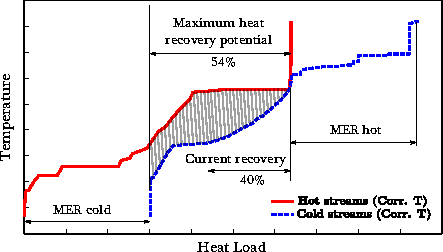
\includegraphics [height=4.3cm]{figures/HeatIntegration/figMERcc.pdf} 
        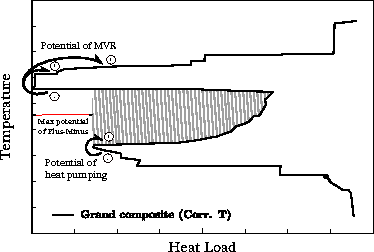
\includegraphics [height=4.3cm]{figures/HeatIntegration/figMERgcc.pdf}
        \caption{Composite and Grand Composite Curves of the process after heat integration}
       \label{fig1:mer}
        \end{center}
        \end{figure}
 
        

Based on the result of the GCC and the plus-minus principle \cite{Linnhoff1993503}, the maximum heat recovery can be further improved by either integrating supplementary equipment (like the heat pump) or by modifying process operating conditions (such as modifying the pressure). The analysis of the GCC in Fig. \ref{fig1:mer}b with respect to the condition of this system (streams phase and temperature range) shows that there is a large potential for the Mechanical Vapor Recompression (MVR) or heat pumping (or both). The compression cycles are added to the appropriate place with respect to the pinch point temperature. This procedure is however possible until a new pinch point would be activated. Therefore, in order to increase the MVR potential while avoiding a quick creation of new pinch points, the heat pumping system is additionally proposed to be integrated with the Composite Curves. Considering the interdependency of the different actions, the flow rates and the selection of the most effective actions are obtained by solving an optimization problem. Obviously, we bear in mind that the implementation of every new solution of the system will modify the target. Suitable energy conversion units are now integrated and their optimum flow rate is found by Mixed Integer Linear Programming (MILP) formulation proposed by \citet{marechal1998process}. This formulation helps define the heat cascade of the Pinch Analysis method as a set of inequality constraints. This model selects the equipments in the superstructure and determines their optimal operating flow rate in the integrated system. The objective is then to minimize the operating costs, including the fuel and the electricity. In order to optimize the mass flow rates of the MVR, a new equality constraint is also added to the MILP optimization problem. The optimal integration of MVR and heat pumps is performed simultaneously with the energy conversion units. The Composite Curves of the system with MVR alone and together with the heat pumps are respectively shown in Fig. \ref{fig1:HPmvr}a and b. By adding an MVR unit, the mechanical power is calculated and a new hot stream is implemented. The principle of the calculation for the MVR is also reported in Fig. \ref{fig1:MVR}. In order to create a link between the part which is recompressed and the part used by the direct heat exchange, the equivalent of the expression $\left( \dot{m}_{total}=\dot{m}_{mvr}+\dot{m}_{dhe}\right) $ is added to the MILP problem as a new constraint \cite{EPFL-ARTICLE-163637}.


      \begin{figure}[h]
      \begin{center}
      \begin{tabular}{cc}
        \subfloat[With MVR]{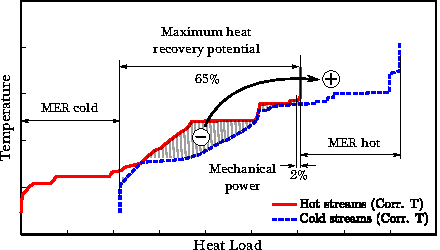
\includegraphics [height=4cm]{figures/HeatIntegration/HPmvr_mvralone.pdf}} & 
        \subfloat[With MVR and HP]{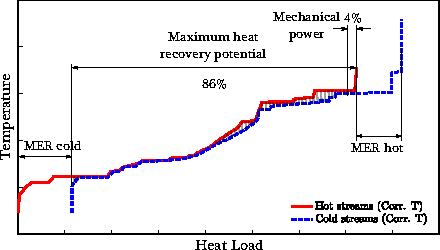
\includegraphics [height=4cm]{figures/HeatIntegration/HPmvr_mvrhp.pdf}}
       \end{tabular}
      \caption{Composite Curves after improvement potentials}
      \label{fig1:HPmvr}
      \end{center}
      \end{figure}
      
 \begin{figure}[h]
 \begin{center}
 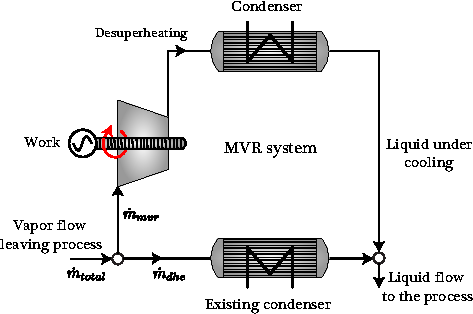
\includegraphics [width=80mm]{figures/HeatIntegration/MVR.pdf}
 \caption{Principle of the MVR integration}
 \label{fig1:MVR}
 \end{center}
 \end{figure}
 
 Adding an MVR unit to transfer the heat from below to above of the pinch, results in the 11\% further improvement of the heat recovery potential (from 54\% in case of the process integration alone to 65\% in case MVR integrated) at the expense of 2\% mechanical power which corresponds to a COP of 5.5. Considering the newly activated pinch points in Fig. \ref{fig1:HPmvr}a, additional heat pumps are also added to system in Fig. \ref{fig1:HPmvr}b in order to further increase the heat recovery potential up to 86\%. This results to 32\% additional heat recovery than the original heat integration opportunities including 4\% of mechanical power requirement. This corresponds to a COP of 8. With the three ideal targets shown here, the overall evaluated energy savings could be between 20\% - 45\% approximately.
          
